\documentclass[student, noshadow, lsr, english, aspectratio=169]{ITR_LSR_slides}
% student options:
% lsr 				-> lsr, template (remove for itr)
% english 			-> enables english language format
% aspectratio=43	-> 4:3 layout

\addbibresource{ref.bib}
\graphicspath{{pics/}{logos/}}

\title{Reasoning Models Can Be Effective Without Thinking - Ma et. al.}
\presenter{Keno Bürger}

\typeofpres{Scientific Seminar Machine Learning}

%\usepackage[bigfiles]{media9} %option bigfiles not needed for xelatex, runs without problems on ubuntu14
%%%%%%%%%%%%%%%%%%%%%%%%%%%%%%%%%%%%%%%%%%%%%%%%%%%%%%%%%%%%%%%%%%%%%%%%%%%%%%%%
\usepackage{multirow}
\usepackage{graphicx}
\usepackage[T1]{fontenc}
\usepackage{lmodern}
\usepackage{tabularx}
\usepackage{enumitem}
\usepackage{adjustbox}
\usepackage{array}
\usepackage{booktabs}
\usepackage{makecell}

\begin{document}


\begin{frame}
    \titlepage
\end{frame}


%%%%%%%%%%%%%%%%%%%%%%%%%%%%%%%%%%%%%%%%%%%%%%%%%%%%%%
\section{Introduction}

\begin{frame}
	\frametitle{Motivation}
	\begin{itemize}
		\item Reasoning models have significantly improved the performance of LLM systems
		\item Include an explicit, lengthy Thinking process at the cost of increased token usage and latency
		\item Paper questions the necessity of this Thinking process
		\item Ongoing research to improve efficiency and effectiveness of reasoning models
		\item Investigates the effectiveness of reasoning models without the Thinking process
	\end{itemize}
\end{frame}

\begin{frame}
    \frametitle{Background Knowledge: Reasoning Models}
    \begin{itemize}
        \item Training Reasoning Models:
            \begin{itemize}
                \item Chain-of-Thought (CoT) Fine-Tuning: Fine-tune models on datasets with explicit reasoning steps to improve interpretability and accuracy
				\item Instruction Tuning: Train models on task-specific instructions to guide reasoning for complex tasks
				\item Reinforcement Learning (RL): Use RL with human feedback (RLHF) to reward correct and interpretable reasoning steps
            \end{itemize}
        \item Key Difference from non-Reasoning Models:
            \begin{itemize}
                \item Reasoning models are explicitly trained to generate intermediate steps, while non-reasoning models rely on implicit patterns in the data
            \end{itemize}
    \end{itemize}
\end{frame}

\begin{frame}
    \frametitle{Background Knowledge: Efficiency in LLMs}
    \begin{itemize}
        \item Efficiency Trade-offs:
            \begin{itemize}
                \item Explicit reasoning improves accuracy but increases latency and token usage
                \item Token-constrained settings require balancing reasoning depth and efficiency
            \end{itemize}
        \item Implicit Reasoning:
            \begin{itemize}
                \item Models generate answers without explicit reasoning steps
            \end{itemize}
        \item Scaling Approaches:
            \begin{itemize}
                \item Sequential Scaling: Processes reasoning steps one at a time, increasing latency but ensuring step-by-step accuracy
                \item Parallel Scaling: Executes multiple reasoning paths simultaneously, reducing latency but requiring more computational resources
            \end{itemize}
    \end{itemize}
\end{frame}

\begin{frame}
    \frametitle{Related Work}
    \begin{columns}
        \column{0.6\textwidth}
        \begin{itemize}
            \item Contrasting prior work, this paper demonstrates competetive performance by disabling the Thinking process
            \item Techniques like CoT and instruction tuning to elicit reasoning abilities in LLMs \cite{huang_towards_2023,ott_thoughtsource_2023,xu_towards_2025}
            \item Ongoing debate about whether LLMs truly reason or simply mimic reasoning patterns from training data \cite{hochlehnert_sober_2025, xu_towards_2025} \newline $\rightarrow$ necessity of explicit reasoning steps?
        \end{itemize}

        \column{0.4\textwidth}
        \centering
        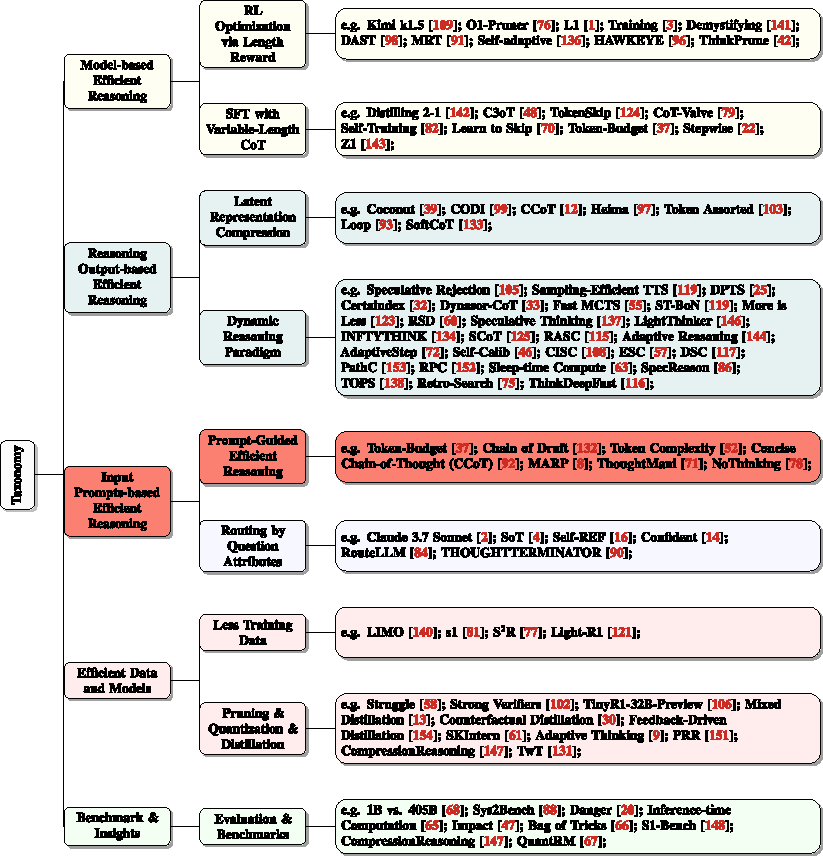
\includegraphics[width=\textwidth]{taxonomy.pdf}
        % \caption{Taxonomy of literature on efficient reasoning}
    \end{columns}
\end{frame}

\begin{frame}
	\frametitle{Main Contribution}
	\begin{itemize}
		\item Identification of NoThinking's \textbf{low-budget superiority}, particularly in token-constrained settings
		\item Development of a \textbf{parallel scaling framework} combining NoThinking with best-of-N sampling, achieving \textbf{7× lower latency} and \textbf{4× less token usage} compared to sequential Thinking approaches
		\item comparable results can be achieved through \textbf{implicit reasoning}
	\end{itemize}
\end{frame}

%%%%%%%%%%%%%%%%%%%%%%%%%%%%%%%%%%%%%%%%%%%%%%%%%%%%%%
\section{Methodology}

\begin{frame}
	\frametitle{Methods and Experimental Setup}
	\centering
	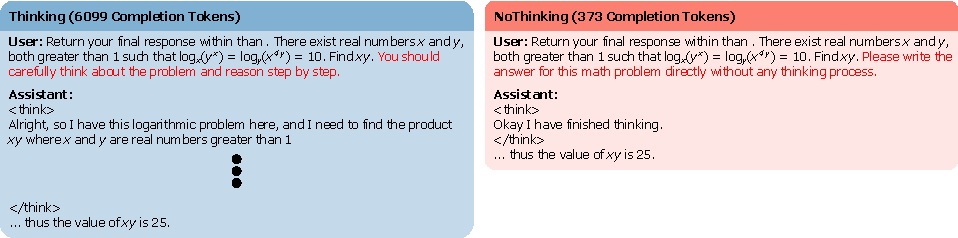
\includegraphics[width=\textwidth]{NoThinking.pdf}
	\begin{itemize}
		\item DeepSeek-R1-Distill-Qwen-32B (additional baseline: Qwen-32B-Instruct)
		\item Budget forcing technique \cite{muennighoff_s1_2025}: average token usage from NoThinking applied to Thinking $\rightarrow$ at this limit model is prompeted to produce a final answer
	\end{itemize}
\end{frame}

\begin{frame}
	\frametitle{DeepSeek-R1-Distill-Qwen-32B}
	\begin{itemize}
		\item First-generation reasoning model from DeepSeek
		\item Distilled from DeepSeek-R1 based on Qwen2.5-32B architecture
		\item Created through sophisticated knowledge distillation process
		\item Two RL stages in teacher model to discover improved reasoning patterns
		\item Two SFT stages to improve reasoning and non-reasoning capabilities
	\end{itemize}
\end{frame}

\begin{frame}
	\frametitle{Benchmarks}
	% \begin{itemize}
	% 	\item Mathematical problem solving
	% 	\begin{itemize}
	% 		\item AIME 2024/AIME 2025: American Invitational Mathematics Examination
	% 		\begin{itemize}
	% 			\item compare different models https://www.vals.ai/benchmarks/aime-2025-03-13
	% 			\item invite only mathematics competition for high-school students in the top 5\% of the AMC 12 mathematics exam
	% 			\item 15 questions, 3 hours, answers are integers from 0 to 999
	% 		\end{itemize}
	% 		\item AMC 2023: American Mathematics Competitions
	% 		\begin{itemize}
	% 			\item 25 questions multiple choice test (5 answers) one is correct
	% 			\item 40 minutes to complete
	% 		\end{itemize}
	% 		\item Olympiad Bench: more advanced reasoning
	% 		\begin{itemize}
	% 			\item https://arxiv.org/abs/2402.14008
	% 			\item Olympiad level bilingual multimodal scientific benchmark featuring 8476 problem from math and physics competitions
	% 		\end{itemize}
	% 	\end{itemize}
	% 	\item Coding
	% 	\begin{itemize}
	% 		\item LiveCodeBench: contamination free evaluation of LLM for LiveCodeBench
	% 		\begin{itemize}
	% 			\item collects new problems over time focusing on broad code related capabilities
	% 			\item leaderboard: https://livecodebench.github.io/leaderboard.html
	% 		\end{itemize}
	% 	\end{itemize}
	% 	\item Formal theorem proving
	% 	\begin{itemize}
	% 		\item MiniF2F: formal mathematical reasoning benchmark
	% 		\begin{itemize}
	% 			\item statements from olympiads (AMC,AIME, IMO) as well as high-school and undergraduate maths classes
	% 			\item work in progress
	% 		\end{itemize}
	% 		\item ProofNet: logic and theorem proving benchmark
	% 		\begin{itemize}
	% 			\item undergraduate level mathematics
	% 			\item 371 examples consisting of formal theorem statements, a natural language theorem statement and a natural language proof
	% 			\item challenging benchmark to drive progess in autoformalization and automatic theorem proving
	% 		\end{itemize}
	% 	\end{itemize}
	% \end{itemize}
	\centering
	\begin{adjustbox}{width=\textwidth, max totalheight=0.85\textheight}
		\begin{tabular}{>{\centering\arraybackslash}m{2.5cm}p{4cm}p{10cm}}
		\Xhline{1pt}
		\textbf{Use Case} & \textbf{Benchmark} & \textbf{Details} \\ \hline
		\multirow{3}{2.5cm}{\centering Mathematical\\Problem\\Solving} 
			& AIME 2024/AIME 2025 & 
			\begin{itemize}[leftmargin=*, nosep, topsep=6pt, partopsep=0pt, before={\vspace{-\baselineskip}}]
				\item 15 questions, 3 hours
				\item Answers are integers from 0 to 999
			\end{itemize} \\ \cline{2-3}
			 & AMC 2023 & 
			\begin{itemize}[leftmargin=*, nosep, topsep=6pt, partopsep=0pt, before={\vspace{-\baselineskip}}]
				\item 25 multiple choice questions, 40 minutes
				\item One correct answer out of 5 choices
			\end{itemize} \\ \cline{2-3}
			 & Olympiad Bench & 
			\begin{itemize}[leftmargin=*, nosep, topsep=6pt, partopsep=0pt, before={\vspace{-\baselineskip}}]
				\item Advanced reasoning benchmark containing math and physics problems
				\item 8476 problems with an sophisticated automated scoring pipeline to verify solutions
			\end{itemize} \\ \hline
		\multirow{1}{2.5cm}{\centering Coding} 
			& LiveCodeBench & 
			\begin{itemize}[leftmargin=*, nosep, topsep=6pt, partopsep=0pt, before={\vspace{-\baselineskip}}]
				\item Contamination-free evaluation of coding abilities
				\item Code execution framework evaluates generated programs against test case
			\end{itemize} \\ \hline
		\multirow{2}{2.5cm}{\centering Formal\\Theorem\\Proving} 
			& MiniF2F & 
			\begin{itemize}[leftmargin=*, nosep, topsep=6pt, partopsep=0pt, before={\vspace{-\baselineskip}}]
				\item Statements from olympiads (AMC, AIME, IMO) and high-school/undergraduate math classes
				\item Formal system proof checkers
			\end{itemize} \\ \cline{2-3}
			 & ProofNet & 
			\begin{itemize}[leftmargin=*, nosep, topsep=6pt, partopsep=0pt, before={\vspace{-\baselineskip}}]
				\item Logic and theorem proving benchmark
				\item 371 examples with formal theorem statements, natural language theorem statements, and proofs.
			\end{itemize} \\
			\Xhline{1pt}
		\end{tabular}
	\end{adjustbox}
\end{frame}

\begin{frame}
	\frametitle{Metrics}
	% \begin{itemize}
	% 	\item pass@k: number of problems solved correctly
	% 	\begin{itemize}
	% 		\item pass@1: number of problems solved correctly with the first attempt
	% 		\item pass@k: number of problems solved correctly with the first k attempts
	% 		\item tackels problem with matching against reference due to limitations in language differences specifically in coding tasks
	% 		\item generate $n \geq k$ solutions and count number of correct samples $c \leq n$ that pass unit tests
	% 	\end{itemize}
	% 	\item Mean and standard deviation of entropy across all questions
	% 	\begin{itemize}
	% 		\item entropy: measure of uncertainty in a probability distribution (model prediction)
	% 		\item higher mean entropy (close to the theoretical maximum): high uncertainty, greater diversity across questions, low variance (small compared to the the mean): more consistent diversity
	% 		\item quantifies how well the model predicts the next word in a sequencs as a model assigns probabilits to possible next words
	% 		\item diversity: range and variability present in the outputs generated by the model (linguistic, representation, conceptual)
	% 	\end{itemize}
	% \end{itemize}
	\begin{itemize}
		\item \textbf{pass@$\mathbf{k}$} measuring the probability of obtaining at least one correct output
		\begin{itemize}
			\item $k$ randomly selected samples, n generated completions, c correct outputs
			\item $\text{pass}@k = \mathbb{E}_{\text{problems}} \left[ 1 - \frac{\binom{n-c}{k}}{\binom{n}{k}} \right]$
		\end{itemize}
		\item \textbf{Mean and standard deviation} of entropy
		\begin{itemize}
			\item entropy: measure of uncertainty in a probability distribution (model prediction)
			\item higher mean entropy (close to the theoretical maximum): high uncertainty, greater diversity across questions
			\item low variance (small compared to the the mean): more consistent diversity
		\end{itemize}
	\end{itemize}
\end{frame}

\begin{frame}
	\frametitle{Scaling}
	\begin{itemize}
		\item \textbf{Parallel Scaling}: Distributes computations across multiple devices to process tasks simultaneously
		% Communication overhead between GPUs can impact runtime.
		\item \textbf{Sequential Scaling}: Executes computations one after another 
		% Effective for reasoning models but potentially computationally expensive.
		\item \textbf{Metrics}: Latency, maximum number of tokens.
		\item \textbf{Perfect verifiers not available}:
		\begin{itemize}
			\item \textit{Confidence-based}: Model's self-certainty (confidence score) in predictions. Methods include highest confidence selection and weighted voting across answers.
			\item \textit{Majority voting}: Selection of the most common response (consensus)
		\end{itemize}
	\end{itemize}
\end{frame}


%%%%%%%%%%%%%%%%%%%%%%%%%%%%%%%%%%%%%%%%%%%%%%%%%%%%%%
\section{Key Results}

\begin{frame}
	\frametitle{Token Efficiency}
	% fig. 5, fig. 6
	\centering
    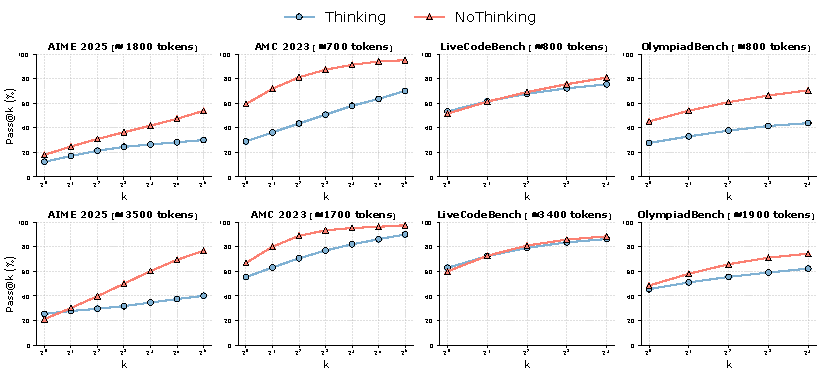
\includegraphics[width=\textwidth]{Fig5_Control.pdf}
\end{frame}

\begin{frame}
	\frametitle{Accuracy}
	% fig. 4
	\centering
    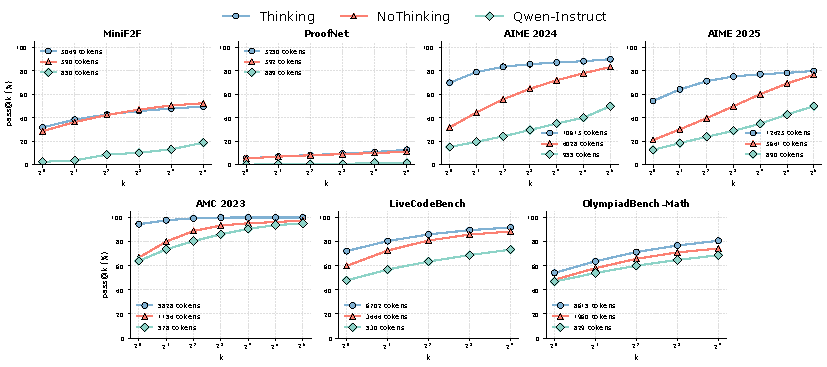
\includegraphics[width=\textwidth]{Fig4_NoControl.pdf}
\end{frame}

\begin{frame}
	\frametitle{Parallel Scaling}
	% fig. 7, tab. 2
	\centering
	\begin{adjustbox}{width=\textwidth, max totalheight=0.85\textheight}
		\begin{tabular}{ccccccc}
			\Xhline{1pt}
			\multirow{2}{*}{\textbf{Task}} & \multirow{2}{*}{\textbf{Thinking}} & \multirow{2}{*}{\textbf{BF (tokens)}} & \multirow{2}{*}{\textbf{Pass@K}} & \multicolumn{3}{c}{\textbf{Selection Methods (Pass@1)}} \\
            \cline{5-7}
            & & & & \textbf{Majority Voting} & \textbf{Confidence + Highest} & \textbf{Confidence + Voting} \\ \hline
			\multirow{2}{*}{AIME 2024} & \textit{Thinking} & 3500 & 73.33 & 43.33 & 40.00 & \textbf{46.67} \\
			& NoThinking & 3500 & 77.30 & 46.67 & 20.00 & \textbf{50.00} \\ \hline
			\multirow{2}{*}{AIME 2025} & \textit{Thinking} & 3500 & 40.00 & \textbf{30.00} & \textbf{30.00} & \textbf{30.00} \\
			& NoThinking & 3500 & 53.73 & \textbf{33.33} & 20.00 & \textbf{33.33} \\ \hline
			\multirow{2}{*}{AMC 2023} & \textit{Thinking} & 2400 & 92.50 & \textbf{77.50} & 65.00 & \textbf{77.50} \\
			& NoThinking & 2400 & 95.00 & 77.50 & 57.50 & \textbf{85.00} \\
			\Xhline{1pt}
		\end{tabular}
	\end{adjustbox}
	\vspace{4pt}
	\begin{itemize}
		\item Improved pass@1 results at similar or lower latency
		\item Reduced token usage for tasks with perfect verifiers
	\end{itemize}
\end{frame}

% \begin{frame}
% 	\frametitle{Stability and Task Specific Observations}
% 	\begin{itemize}
% 		\item The paper shows that reasoning models can be effective without thinking
% 		\item It provides a new perspective on the effectiveness of reasoning models
% 		\item The results show that reasoning models can be effective in various scenarios
% 	\end{itemize}
% \end{frame}

%%%%%%%%%%%%%%%%%%%%%%%%%%%%%%%%%%%%%%%%%%%%%%%%%%%%%%
\section{Analysis \& Discussion}

\begin{frame}
	\frametitle{Analysis}
	\centering
    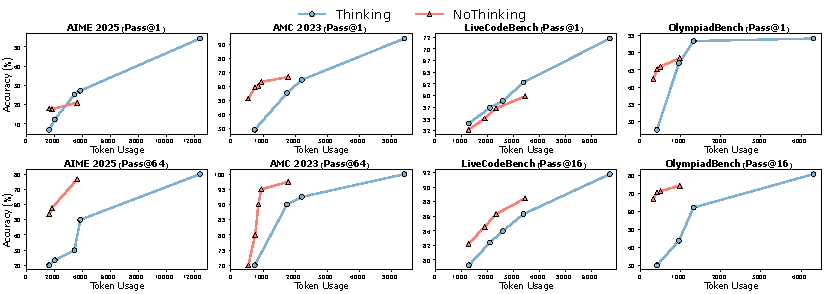
\includegraphics[width=\textwidth]{Fig6_Result.pdf}
	\begin{itemize}
		\item In low-budgt settings, NoThinking outperforms Thinking %especially as the number of k increases
		\item Parallel scaling $\rightarrow$ improved accuracy-latency tradeoff%reduces latency, 
	\end{itemize}
\end{frame}

\begin{frame}
	\frametitle{Discussion}
	\centering
	\begin{adjustbox}{width=\textwidth, max totalheight=0.85\textheight}
		\begin{tabular}{p{0.48\textwidth}p{0.48\textwidth}}
			\Xhline{1pt}
			\textbf{Strengths} & \textbf{Limitations} \\ \hline
			\begin{itemize}
				\item Broad evaluation %well supported by benchmarks and metrics
				\item Analysis of different scaled models
				\item Efficiency gains
				\item Practical Applications with parallel scaling
			\end{itemize} &
			\begin{itemize}
				\item Poor performance at pass@1 and Coding
				\item Results limited to one model %model specific behavior?
				\item No interpretive/subjective/humaties-style tasks
				\item No ablation studies on different components %testing different prompts
				\item Raw performance still favors large models
			\end{itemize} \\ 
			\Xhline{1pt}
		\end{tabular}
	\end{adjustbox}
	\vspace{4pt}
	\begin{itemize}[label=$\Rightarrow$] 
		\item Peer review and test on general conversation/common sense reasoning tasks
		\item Applications with strict latency or cost constraints
	\end{itemize}
\end{frame}

%%%%%%%%%%%%%%%%%%%%%%%%%%%%%%%%%%%%%%%%%%%%%%%%%%%%%
\begin{frame}[allowframebreaks]
    \frametitle{References}
    \nocite{*} 
    \printbibliography[heading=none]
\end{frame}

\end{document}
